% -*- mode:flyspell; mode:latex -*-
\documentclass[12pt]{article}

% \addtolength{\oddsidemargin} {-0.885in}
% \addtolength{\textwidth}{1.75in}
% \addtolength{\evensidemargin}{-0.8in}
% topmargin -0.5in
\usepackage[a4paper, top=1cm, left=1.5cm, right=1.5cm]{geometry} % width= , 

\usepackage[latin1]{inputenc}
\usepackage[T1]{fontenc}
\usepackage[english]{babel}
\usepackage{graphicx}
\usepackage{float}


\usepackage{tikz}
\usepackage{[caption}
\usetikzlibrary{arrows}
\usetikzlibrary{decorations.markings}
\usetikzlibrary{decorations.pathmorphing}
% \usepackage[absolute,overlay]{textpos}
% \usepackage{onimage}

\usepackage{times}
\usepackage{graphics}

% \usepackage{subfigure}
% \usepackage{scalefnt}
%
% \renewcommand\thesubfigure{\arabic{subfigure}}

\usepackage{amsmath}
\usepackage{hyperref}
\usepackage{hhline}
\usepackage{subfig}
\usepackage{color}
\usepackage[all]{hypcap}

\usepackage[normalem]{ulem}  % for striking out
% \usepackage{fancyhdr}
% \pagestyle{fancy}
% \fancyhead[C]{}
% \fancyhead[L] {\it{Mu2e-doc-29670-v1.0} }
%%%%%%%%%%%%%%%%%%%%%%%%%%%%%%%%%%%%%%%%%%%%%%%%%%%%%%%%%%%%%%%%%%%%%%%%%%%%%%
% use natbib - biblatex not available on Mu2e interactive nodes
%%%%%%%%%%%%%%%%%%%%%%%%%%%%%%%%%%%%%%%%%%%%%%%%%%%%%%%%%%%%%%%%%%%%%%%%%%%%%%
\usepackage[square,sort,comma,numbers]{natbib}

% location of the .bib files: env var BIBINPUTS (~/library/bibliography)

% \usepackage[backend=biber, style=numeric-comp, sorting=ynt] {biblatex}
% \addbibresource{clfv.bib}

% \addbibresource{stntuple.bib}
% \addbibresource{mu2e_web.bib}
% \addbibresource{radiative_pion_capture.bib}

\graphicspath{{figures/}}
%%%%%%%%%%%%%%%%%%%%%%%%%%%%%%%%%%%%%%%%%%%%%%%%%%%%%%%%%%%%%%%%%%%%%%%%%%%%%%
% for portability, make sure all commands are included locally
% order them alphabetically
%%%%%%%%%%%%%%%%%%%%%%%%%%%%%%%%%%%%%%%%%%%%%%%%%%%%%%%%%%%%%%%%%%%%%%%%%%%%%%
% \include{commands}

\newcommand {\keVc}       {\mbox{$\rm keV\!/\!c$}}
\newcommand {\kmax}       {\mbox{$k_{\rm max}$}}

\newcommand {\MeVc}       {\mbox{$\rm MeV\!/c$}}
\newcommand {\MeVcsq}     {\mbox{$\rm MeV\!/c^2$}}

\newcommand {\mumemconv}[1][A] {\mbox{$\mu^- \textrm{#1} \rightarrow e^- \textrm{#1}$}}
% Define a relay to have 2 default arguments instead of limit of 1
\newcommand {\mumepconv}[1][A] {%
  \def\ArgI{{#1}}%store the first argument
  \mumepconvRelay
}
\newcommand \mumepconvRelay[1][A]  {\mbox{$\mu^- \textrm{\ArgI} \rightarrow e^+ \textrm{#1}$}}
\newcommand {\muminus}    {\mbox{$\mu^-$}}
\newcommand {\muplus}    {\mbox{$\mu^+$}}
\newcommand {\MuToEm}     {\mbox{$\mu^- \ra e^-$}}
\newcommand {\MuToEp}     {\mbox{$\mu^- \ra e^+$}}
\newcommand {\MuPToEp}    {\mbox{$\mu^+ \ra e^+$}}
\newcommand {\ra}        {\rightarrow}
\newcommand {\tandip}    {\mbox{$\tan \lambda$}}

\newcommand {\Pb}[1]     {\mbox{$\rm ^{#1}Pb$}}                 % isotopes of lead
\newcommand {\Au}[1]     {\mbox{$\rm ^{#1}Au$}}                 % isotopes of gold
\newcommand {\Ir}[1]     {\mbox{$\rm ^{#1}Ir$}}                 % isotopes of iridium
%%%%%%%%%%%%%%%%%%%%%%%%%%%%%%%%%%%%%%%%%%%%%%%%%%%%%%%%%%%%%%%%%%%%%%%%%%%%%%
% editing commands
%%%%%%%%%%%%%%%%%%%%%%%%%%%%%%%%%%%%%%%%%%%%%%%%%%%%%%%%%%%%%%%%%%%%%%%%%%%%%%
\newcommand {\add}[1]    {{\red #1}}
\newcommand {\alt}[1]    {{\green #1}} %alternate comment color
\newcommand {\del}[1]    {{\blue \sout{#1}}}
\newcommand {\dlt}[1]    {{\violet \sout{#1}}} %alternate delete color

\newcommand {\black}     {\color{black}}
\newcommand {\red}       {\color{red}}
\newcommand {\blue}      {\color{blue}}
\newcommand {\strike}[1] {{\blue \sout{#1}}}
%%%%%%%%%%%%%%%%%%%%%%%%%%%%%%%%%%%%%%%%%%%%%%%%%%%%%%%%%%%%%%%%%%%%%%%%%%%%%%
\begin{document}

\begin{titlepage}
  \begin{flushright}
    \bf {MU2E/PHYSICS/xxxxx} \\
    version 1.0
    \today
 \end{flushright}

  \vspace{1cm}

  \begin{center}
    {\Large \bf Commissioning of the Mu2e Data AcQuisition system and the Vertical Slice Test of the straw tracker

      \vspace{0.3in}

      11. Mu2e ROC simulation
    }

    \vspace{1cm}
%     S. Gamba  \footnote{\texttt{Fermilab; e-mail:s.gamba2\@studenti.unipi.it} (University of Pisa)
%     P. Murat \footnote{\texttt{Fermilab; e-mail: murat\@fnal.gov} (FNAL)

   
    version 1.0
    \today
 \end{center}

  \begin{abstract}
    This note presents an analysis of data coming from the teststand of the motherboard and the comparison with ROC simulation.
    \vspace{0.2in}
  \end{abstract}

\end{titlepage}
% \frontmatter
% \chapter*{Abstract}
%
% \addcontentsline{toc}{chapter}{Abstract}
%
% \mainmatter
%
{\tableofcontents}

%%%%%%%%%%%%%%%%%%%%%%%%%%%%%%%%%%%%%%%%%%%%%%%%%%%%%%%%%%%%%%%%%%%%%%%%%%%%%%%
%\chapter{Calibration}
%%%%%%%%%%%%%%%%%%%%%%%%%%%%%%%%%%%%%%%%%%%%%%%%%%%%%%%%%%%%%%%%%%%%%%%%%%%%%%%
% \input{input_data}

%%%%%%%%%%%%%%%%%%%%%%%%%%%%%%%%%%%%%%%%%%%%%%%%%%%%%%%%%%%%%%%%%%%%%%%%%%%%%%%
\newpage
\section {Notes for the authors}
\subsection {Revision history} 
\begin{itemize}
\item
  v1.01: initial version
\end{itemize}

%%%%%%%%%%%%%%%%%%%%%%%%%%%%%%%%%%%%%%%%%%%%%%%%%%%%%%%%%%%%%%%%%%%%%%%%%%%%%%
\section {Introduction to the analysis}

In this note, we present an analysis of the data derived from the readout teststands of the motherboard.
This analysis was performed with the aim of characterizing the functionality of the Data Acquisition (DAQ) system.
A signal generator was employed to send pulses and we tried to understand the output and non-output of the DTC. 
Our study centered on testing the performance of ROCs and DTCs, actually we were reading 1 ROC (96 channels), 
which is the equivalent of one panel or 2 ROCs. The analysis was executed employing a single DTC.
During the analysis, we had the capability to change different generator's features. We varied the event
window duration between successive pulses and modulated the generator's operating frequency. 
Specifically, we could operate with two distinct frequencies: 31.29 MHz/(2$^7$+1), resulting in approximately 250 kHz,
and 31.29 MHz/(2$^9$+1), 60 kHz. \\
The selection of the event window duration and the frequency played an important role in determining the number of hits per event,
considering that the ROC buffer possessed a storage capacity for up to 255 hits. The relationship between the generator 
and readout counts can be summarized as follows:
\begin{itemize}
    \item $N_{gen} \ < \ $255: $N_{readout} \ = \ N_{gen}$;
    \item $N_{gen} \ \geq \ $255: $N_{readout} \ = \ 255$.
\end{itemize}
\section{Monte Carlo simulation}\label{MonteCarlo}
To ensure a comprehensive understanding of our system, we initiated a Monte Carlo Simulation of our Data Acquisition (DAQ) system. 
Given that the maximum allowable number of hits per event is 255, the simulation protocol adheres to the following sequential steps:
\begin{itemize}
  \item Within a time interval ranging from 0 $\mu$s to the reciprocal of the generator frequency, we generated the first event ($t_0$) by following a uniform distribution;
    \item After verified that hits from the same channel, are separated by an interval equivalent to the reciprocal of the generator frequency, we proceeded to 
      generate the second event ($t_1$) by summing this specific time increment to $t_0$;
      \item Subsequently, we verified whether the second pulse remained within the predefined time window. If it did, we included this hit in the ongoing event under construction;
      \item The process of event creation continued until the count of hits reached the maximum threshold of 255, at which point the event construction was terminated.
\end{itemize}
Furthermore, the simulation accounts for the channel to channel and FPGA to FPGA delays. 
This comprehensive approach ensures a faithful representation of the real-world operational aspects of the DAQ system.
\section{Full buffer mode: RUN281}
%%%%%%%%%%%%%%%%%%%%%%%%%%%%%%%%%%%%%%%%%%%%%%%%%%%%%%%%%%%%%%%%%%%%%%%%%%%%%%
\subsection{Time distribution}
The analysis started analyzing the data time distribution of each channel.
After a preliminary observation of the distributions, we saw a different patterns for channels in the first FPGA and in the second FPGA,
as illustrated in Fig. \ref{fig:1}: the initial though  was the occurrence of a cessation in data acquisition for specific channels at a certain time.

\begin{figure}[H]
  \hspace{-0.5in}
  \begin{tikzpicture}
    \node[anchor=south west,inner sep=0] at (0,0.) {
      % \node[shift={(0 cm,0.cm)},inner sep=0,rotate={90}] at (0,0) {}
      % \makebox[\textwidth][c] {
      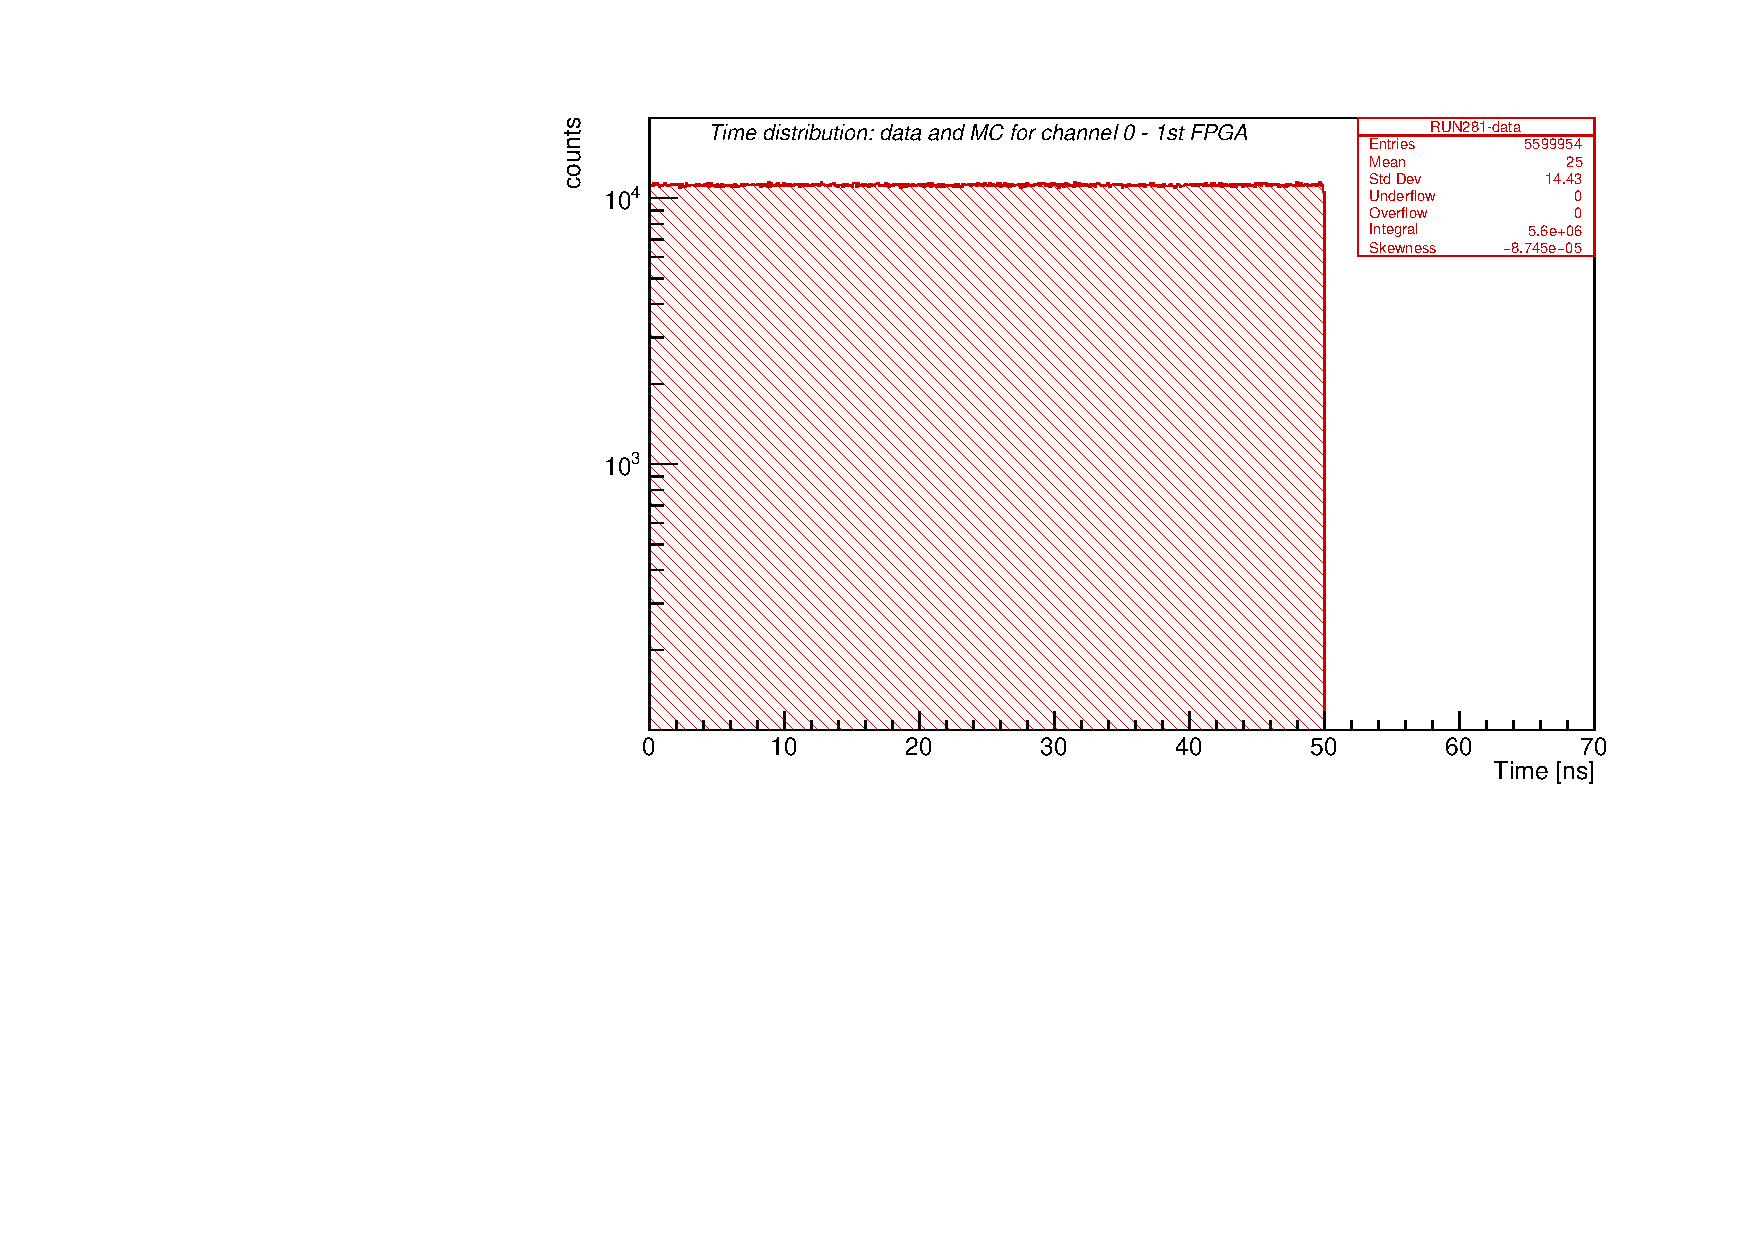
\includegraphics[width=0.5\textwidth]{figures/pdf/figure_00007_timedistr_roc_simulation_ch0}
      % }
    };
    \node[anchor=south west,inner sep=0] at (10,0.) {
      % \node[shift={(0 cm,0.cm)},inner sep=0,rotate={90}] at (0,0) {}
      % \makebox[\textwidth][c] {
      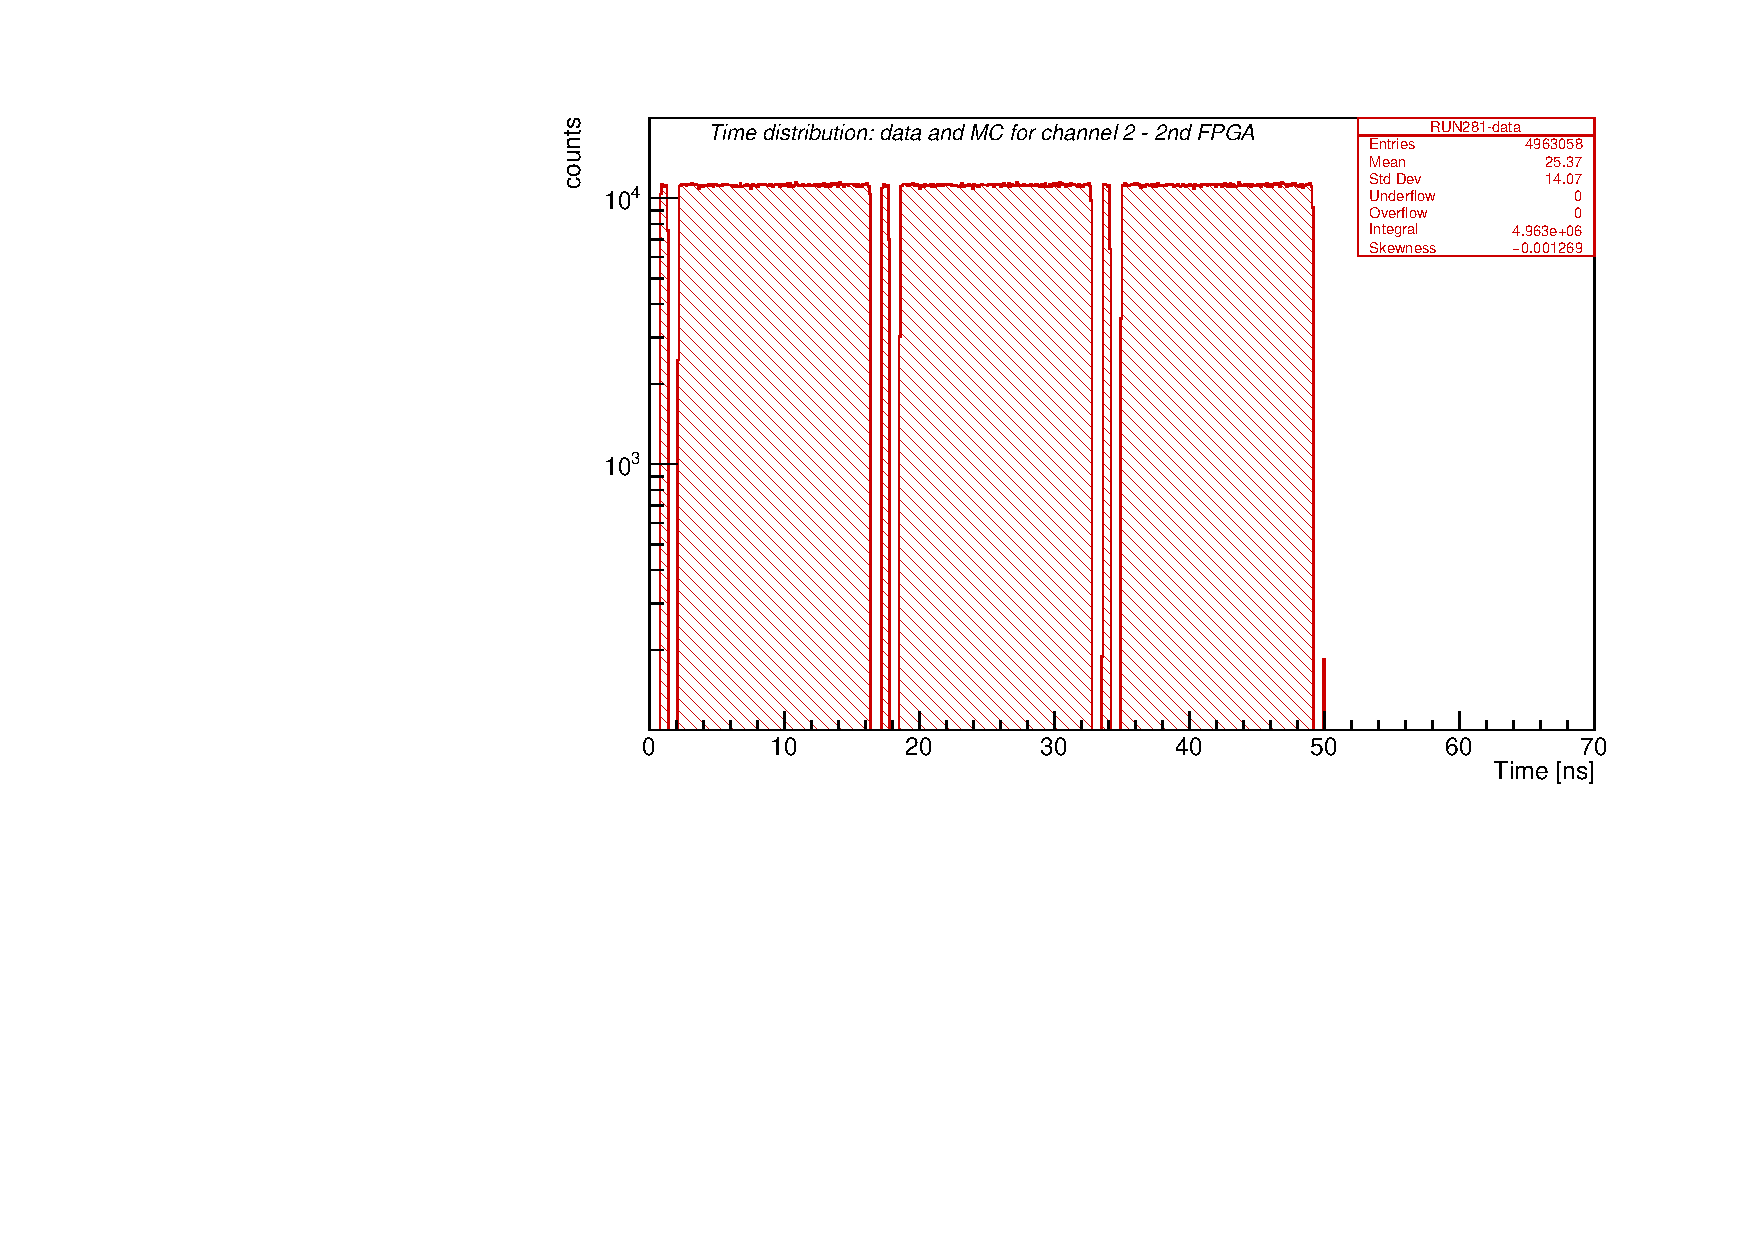
\includegraphics[width=0.5\textwidth]{figures/pdf/figure_00003_timedistr_roc_simulation_ch2}
      % }
    };
  \end{tikzpicture}
  \caption{
    \label{fig:1}
    right: First FPGA's channel time distribution, left: Second FPGA's channel time distribution.
  }
\end{figure}
We thought it was necessary to characterize the apparatus with a Monte Carlo simulation for our Data Acquisition (DAQ) system, in order to understand the interruptions,
so we redirect to section \ref{MonteCarlo} for further information.
\subsection{nh vs ch}
We conducted an analysis by plotting the number of hits in each channel as a function of the channel number, which revealed a non-uniform distribution. 
Specifically, channels were arranged in an ascending order, spanning from channel 0 to channel 95.
As second step, we managed to generate a histogram with an alternative channel order, as we would expect the filling to occur.
Our expectation was to observe a declining trend in the number of hits per channel, primarily due to the progressive filling of the buffer. 
However, contrary to our initial hypothesis, we encountered a distinctive pattern in which the number of hits exhibited a decrease until reaching zero hits at a specific channel,
followed by a subsequent increase beyond the 72nd channel, which corresponds to channel 95.

Upon careful examination, we deduced that the initial channel ordering was incorrect. 
The first and the second lanes of the second FPGA were inverted and also some channels of the second FPGA.
Consequently, we have identified a revised channel sequence, verified also by the Monte Carlo simulation, which is as follows:
\begin{center}
\begin{tabular}{cc}
\textbf{FIST FPGA}: & \\
&91,85,79,73,67,61,55,49,\\
\textit{lane 1}: &43,37,31,25,19,13,7,1,\\
&90,84,78,72,66,60,54,48,\\
& \\
&42,36,30,24,18,12,6,0,\\
\textit{lane 2}: &93,87,81,75,69,63,57,51,\\
&45,39,33,27,21,15,9,3,\\
\textbf{SECOND FPGA}:&\\
&\\
&38,44,5,11,17,23,29,35,\\
\textit{lane 1}:&41,92,2,8,14,20,26,32,\\
&86,80,74,68,62,56,50,47,\\
 & \\
&95,89,83,22,16,28,34,40,\\
\textit{lane 2}:&46,53,59,65,71,77,10,4,\\
&94,88,82,76,70,64,58,52\\
\end{tabular}
\end{center}   
At this point we have plotted the number of hits versus the channel number in the order that the filling occurred, as we can see in Fig. \ref{fig:2}.
\begin{figure}[!h]
\centering
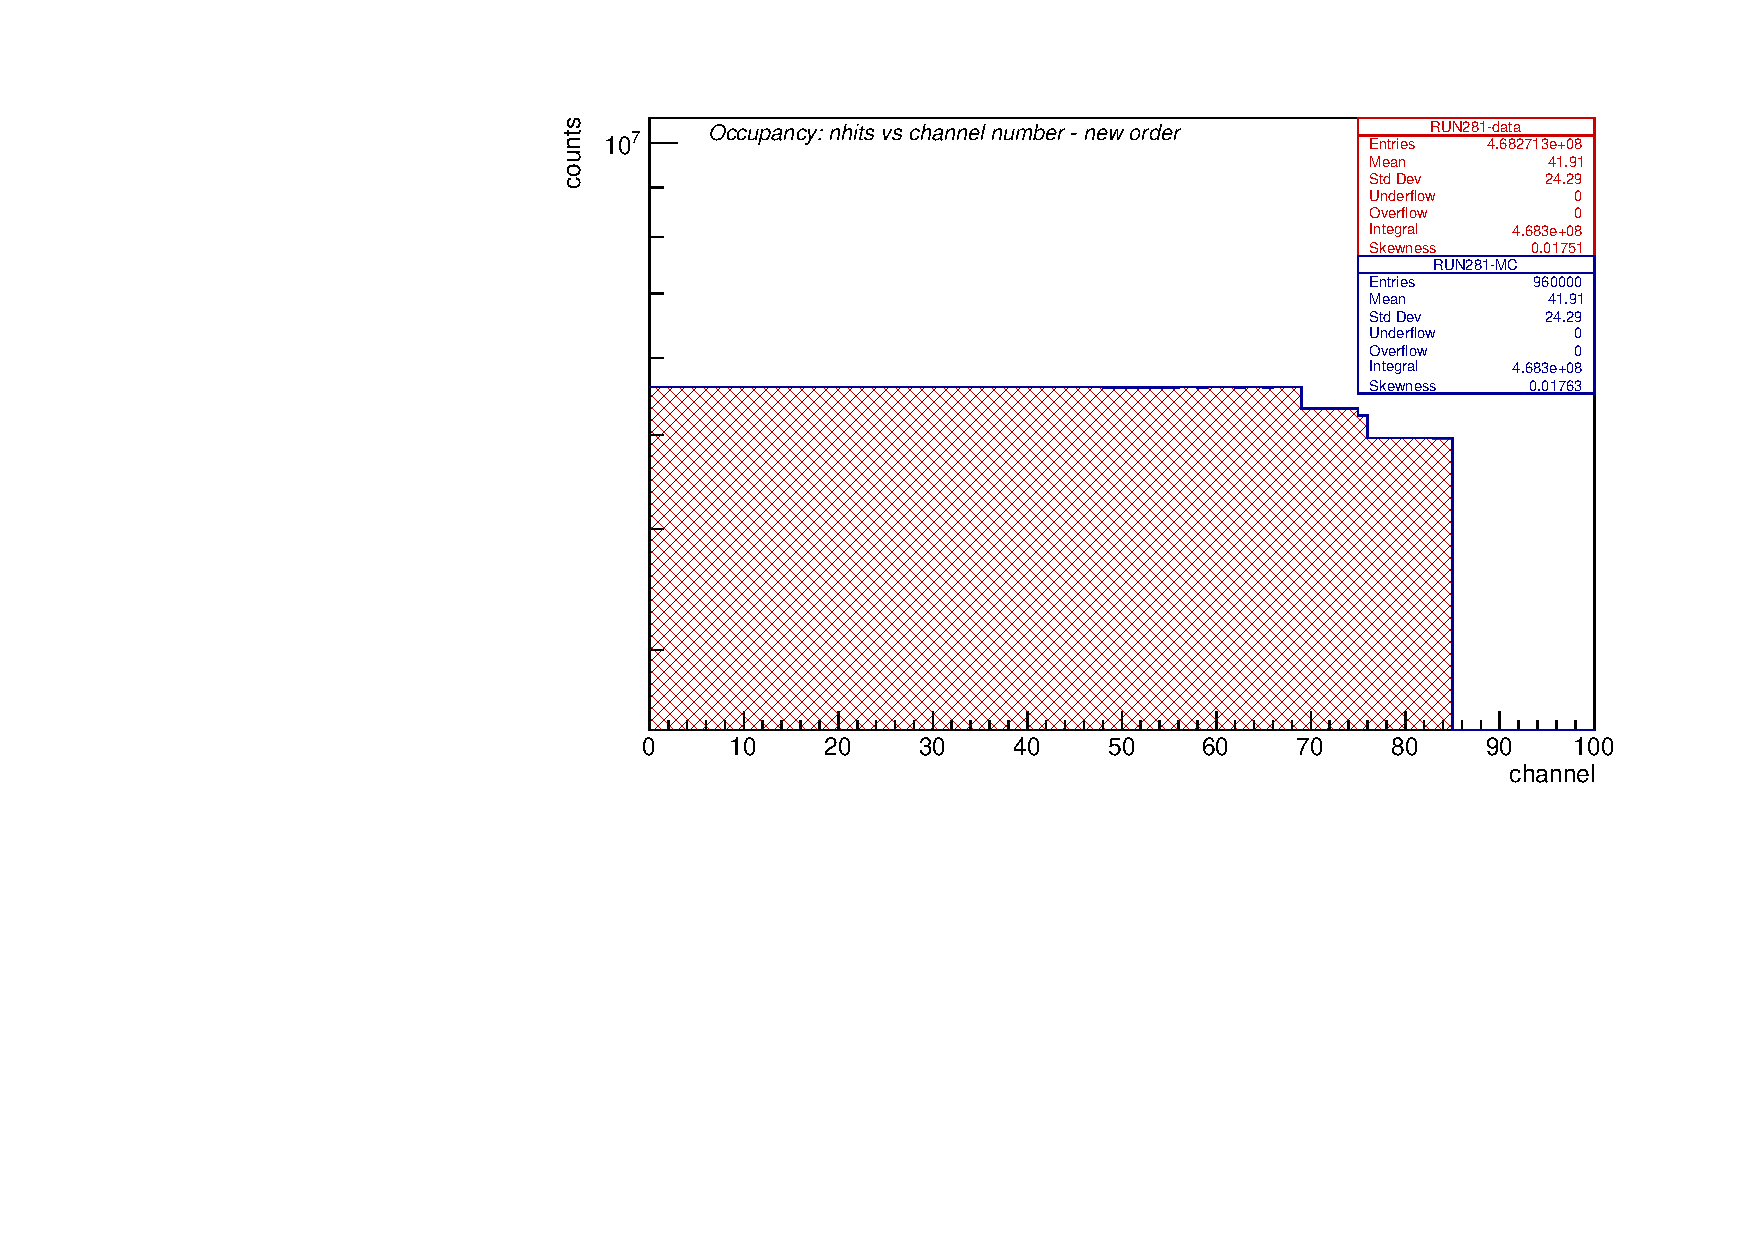
\includegraphics[width =0.8\textwidth]{pdf/figure_00004_nhitsvschannel_roc_simulation_2}
\caption{Occupancy: number of hits versus channel. The ordering of channels adheres to the sequence prescribed by the Monte Carlo simulation.}
\label{fig:2}
\end{figure}
We can see a perfect adherence between data and simulation. We can interpret the histogram as it follows: the initial group of channels in the histogram,
corresponds to the ones in which we accumulate 4 hits (associated with the first FPGA) and 3 hits (associated with the second FPGA). 
Subsequently, we observe a contrasting group of channels where the pattern reverses, 3 hits from the first FPGA followed by 4 hits from the second FPGA.
We can observe a little jump in the middle and it is due to channel to channel time differences.
Time differences are three order of magnitude less than the FPGA ones, so these little jumps are very few, in our case only one appears.
Lastly, the concluding cluster of channels is comprised of those collecting 3 hits from the first FPGA and 3 hits from the second FPGA.



\subsection{nhits}

\section{buffer not full}
\subsection{Time distribution}
\subsection{nh vs ch}
\subsection{nhits}

\section{rate}









%%%%%%%%%%%%%%%%%%%%%%%%%%%%%%%%%%%%%%%%%%%%%%%%%%%%%%%%%%%%%%%%%%%%%%%%%%%%%%
\newpage
\section{Summary}
Upper bounds on the direct beam-related backgrounds are as follows:
\begin{itemize}
\item
  background from beam electrons scattered in the stopping target < $1 \times 10^{-3}$
\item
  background from muon decay in flights < $1 \times 10^{-3}$
\item
  background from beam muons scattered in the stopping target < $1 \times 10^{-5}$
\end{itemize}
%%%%%%%%%%%%%%%%%%%%%%%%%%%%%%%%%%%%%%%%%%%%%%%%%%%%%%%%%%%%%%%%%%%%%%%%%%%%%%
%
%%%%%%%%%%%%%%%%%%%%%%%%%%%%%%%%%%%%%%%%%%%%%%%%%%%%%%%%%%%%%%%%%%%%%%%%%%%%%%
\newpage
\bibliographystyle{unsrtnat}
\bibliography{local,clfv,dio,mu2e_internal_notes}

\end{document}

